\documentclass[twoside,12pt]{article}
\usepackage{amsmath,amsfonts,amsthm,fullpage}
%\usepackage{algorithm}
\usepackage{algorithmic}
\usepackage{float}
\usepackage{graphicx}
\usepackage{listings}
\usepackage[utf8]{inputenc}
\usepackage[vlined, ruled, boxed]{algorithm2e}
\title{Programming Assignment 2}
\author{Han Dongmin, Yuanlai Zhou and Chong Ye}

\begin{document}

\maketitle
\section{Problem Statement}
In this programming assignment, we need to develop a parallel back-tracking algorithm to place n-queens on a $ n * n $ chessboard according to rules. Queens are not allowed to be placed in the same rows/columns or diagonal directions. Both sequential and parallel algorithms need to be designed to find all the correct configurations of the placement. One solution to the problem are represented by an array of $ n $ numbers, $ sol[0,1,2,...,n-1] $, where $ sol[i] $ represents the column where the queen in row $ i $ is placed.
\section{Algorithm}


\subsection{seq\_solver}
We implemented recursive back-tracking algorithm in the sequential calculation. There are two helper functions used in here, \textit{isValid} and \textit{actual\_seq\_solver}.\\
Function \textit{isValid} determines if the current placement would threaten the queens already placed. Specifically, if we are planning to place the queen of row $ i $ in column $ j $, we need to check if the queen will threaten the queens of row $ 0,1,2,...,i-2 $ which are already placed. If not, the function would return \textit{true}. otherwise, return \textit{false}. \\
Function \textit{actual\_seq\_solver} implements the back-tracking algorithm to place the n-queens.The queens are placed row by row, after placing the queen of row $ i $, the function proceeds to place the queen of row $ i+1 $. After a solution is found, the function proceeds to find another feasible placement until all the correct configurations are found. 

\subsection{nqueen\_master}
Master processor (rank 0) implements backtracking to calculate the first $ k $ queens' positions, and sends out the tasks of solving the remaining solutions to this sub-problem $ S_k $ to the workers. The master dispatches one task at a time to available workers. While waiting for the responses from workers, master prepares the next feasible configuration of placing the first $ k $ queens for efficiency. After the worker finishes its work, master dispatches another partial solution to this available worker till all the partial solutions are found. After all the partial solutions are found and all the workers finish their jobs, master sends out the termination signal to terminate the parallel running.\\
Two main helper functions are defined here, $ next\_partial\_solution $ and $ check\_worker\_idle $. The helper function $ next\_partial\_solution $ is used to find the next partial solutions by backtracking algorithm, if a partial solution is found, returns \textit{true}. Then the partial solution would be dispatched to the available worker. The function returns \textit{false} after all the partial solutions are found. The function $ check\_worker\_idle $ returns true if all the workers have finished the jobs. Then the master sends out the termination signal to terminate the parallel running.

\subsubsection{nqueen\_worker}
Workers receive two kinds signals from the master, one is partial solution of placing the first $ k $ queens, the other is the termination signal. If the received signal is partial solution, then the worker needs to finish placing the remaining $ n-k $ queens. The helper function $ worker\_solver $ is defined to find the remaining solutions to the subproblem. The $ worker\_solver $ continues to place the queen of row $ k $ to row $ n-1 $. As soon as one solution is found, the worker sends out the solution to master and then checks if there are other solutions. If all the remaining solutions are found the the subproblem, the worker sends out job finished signal to master and waits for another job. \\
If the work receives termination signal from master, the function would just return.

\section{Optimization}
\subsection{edge cases}
\begin{enumerate}
	\item $ p = 1 $ \\
	When we only use one processor, it means sequential computing. 
	\item $ k = n $ \\
	It means the master processor calculates the solutions of placing $ n $ queens, which simply represents the full solutions. Thus we use sequential algorithm for this case.	
	\item $ k = 0 $ \\
	It means the master does not need to place any queens, thus the workers need to place the queens of row $ 0 $ to row $ n-1 $.
		
\end{enumerate}

\subsection{computation-communication overlap}
We use non-blocking \textbf{MPI\_Irecv} at the master processor side to receive the responses from workers. In this case, the master processor could prepare the next partial solution and have it ready while waiting for the response from workers. As soon as the worker returns solutions and is available, the master hands out the prepared partial solution to the worker, saving the worker's idle waiting time. 


\section{Implementation and Analysis}
\subsection{vary n with fixed p and k}
	With fixed $ p = 8, k = 4 $, we varied the problem size $ n $ from 8 to 16. The runtime versus the problem size is shown below.
	\begin{figure}[H]
		\centering
		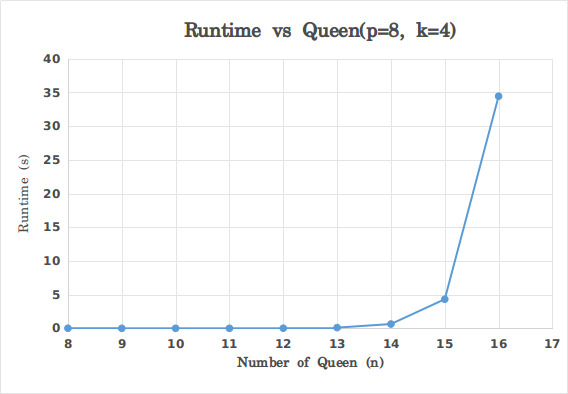
\includegraphics[width=0.6\textwidth]{runVSn}
		\caption{Runtime VS problem size}
	\end{figure}
	
\subsection{vary p with fixed n and k}
	With fixed  $ n = 15, k = 5 $, we varied the number of processors from 1 to 16. The running time versus the number of processors is shown in Figure 1. \\
	\begin{figure}[H]
		\centering
		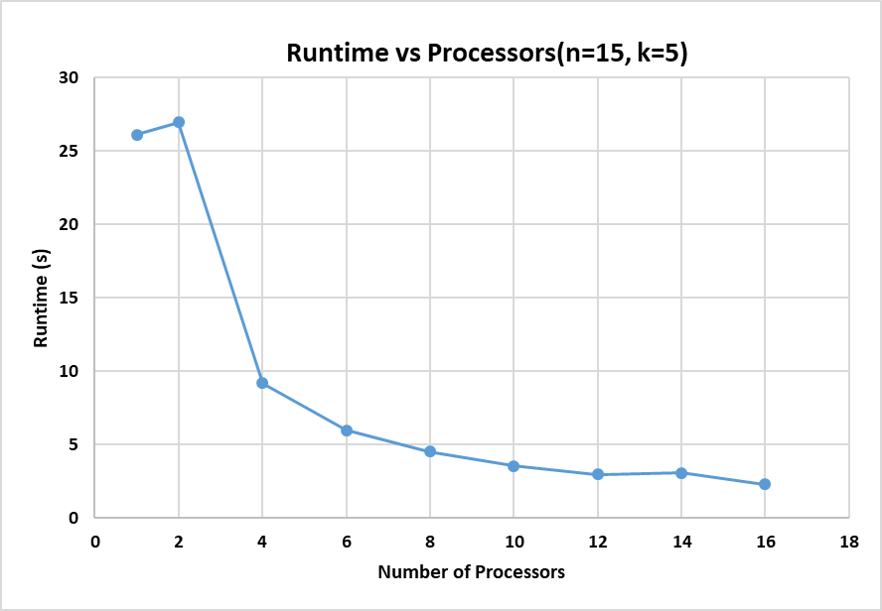
\includegraphics[width=0.6\textwidth]{pVSTime1}
		\caption{Running time VS number of processors}
	\end{figure}
    The speedup and efficiency versus the number of processors are shown in Figure 2 and Figure 3 respectively.
    \begin{figure}[H]
    	\centering
    	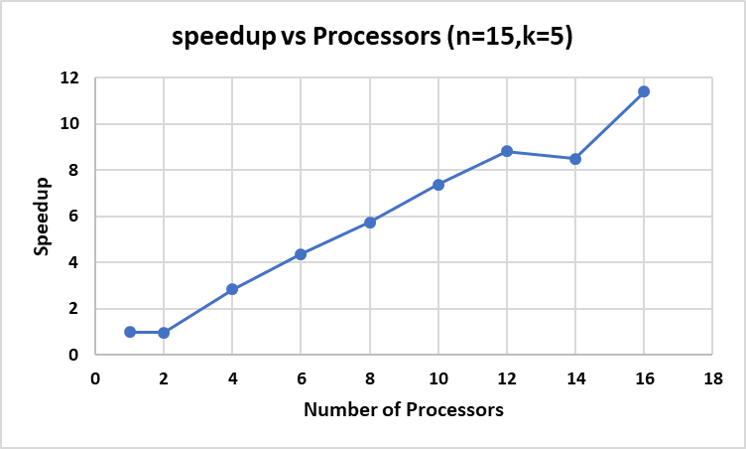
\includegraphics[width=0.6\textwidth]{speedupVSp}
    	\caption{Speedup VS number of processors}
    \end{figure}
   
    \begin{figure}[H]
	\centering
	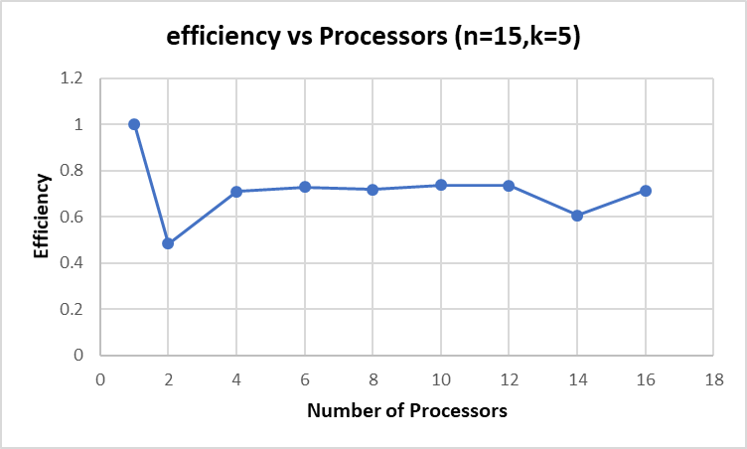
\includegraphics[width=0.6\textwidth]{effiVSp}
	\caption{Efficiency VS number of processors}
    \end{figure}


\subsection{vary k with fixed n and p}
    With fixed $ n = 16, p = 8 $, we varied the problem size of subproblem initialized by the master from 1 to 16. The runtime versus the number of partial solution size is shown in Figure 5.
	\begin{figure}[H]
	\centering
	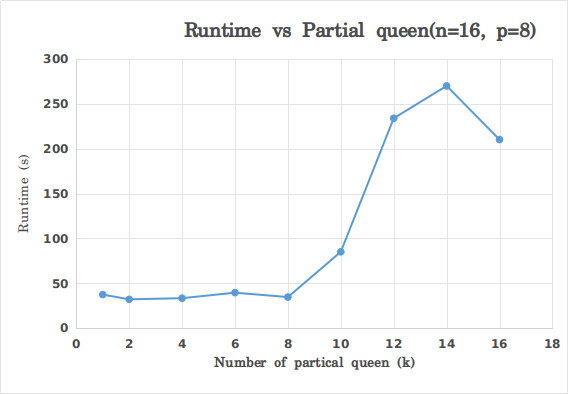
\includegraphics[width=0.6\textwidth]{runVSk}
	\caption{Runtime VS partial solution size}
    \end{figure}

\subsection{largest n with  p = 16 }
\begin{center}
	\begin{tabular}{ |c| c |c|}
		\hline
		n & k & runtime [sec] \\
		\hline
		18 & 3 & 881.989 \\
		\hline
		18 & 4 & 891.974 \\
		\hline
		18 & 5 & 875.629 \\
		\hline
		18 & 6 & 928.418 \\
		\hline
		18 & 7 & 953.889 \\
		\hline
		
	\end{tabular}	
\end{center}
In the limit of 30 minutes, the largest $ n $ we can solve is 18. We solve it with different $ k $ values and found that $ k = 5 $ gives the smallest running time.

\section{Results and Conclusion}
For this programming assignment, we implemented parallel backtracking algorithm for the n-queens problem. We enhanced the understanding of scalability, communication time and computing time of parallel computing and MPI implementation. We also got some interesting findings as discussed in the above analysis section. 

     
\end{document}